%\VignetteIndexEntry{faoswsSeed: A package for the imputation of the seed domain for the Statistical Working System}
%\VignetteEngine{knitr::knitr}
\documentclass[nojss]{jss}\usepackage[]{graphicx}\usepackage[]{color}
%% maxwidth is the original width if it is less than linewidth
%% otherwise use linewidth (to make sure the graphics do not exceed the margin)
\makeatletter
\def\maxwidth{ %
  \ifdim\Gin@nat@width>\linewidth
    \linewidth
  \else
    \Gin@nat@width
  \fi
}
\makeatother

\definecolor{fgcolor}{rgb}{0.345, 0.345, 0.345}
\newcommand{\hlnum}[1]{\textcolor[rgb]{0.686,0.059,0.569}{#1}}%
\newcommand{\hlstr}[1]{\textcolor[rgb]{0.192,0.494,0.8}{#1}}%
\newcommand{\hlcom}[1]{\textcolor[rgb]{0.678,0.584,0.686}{\textit{#1}}}%
\newcommand{\hlopt}[1]{\textcolor[rgb]{0,0,0}{#1}}%
\newcommand{\hlstd}[1]{\textcolor[rgb]{0.345,0.345,0.345}{#1}}%
\newcommand{\hlkwa}[1]{\textcolor[rgb]{0.161,0.373,0.58}{\textbf{#1}}}%
\newcommand{\hlkwb}[1]{\textcolor[rgb]{0.69,0.353,0.396}{#1}}%
\newcommand{\hlkwc}[1]{\textcolor[rgb]{0.333,0.667,0.333}{#1}}%
\newcommand{\hlkwd}[1]{\textcolor[rgb]{0.737,0.353,0.396}{\textbf{#1}}}%

\usepackage{framed}
\makeatletter
\newenvironment{kframe}{%
 \def\at@end@of@kframe{}%
 \ifinner\ifhmode%
  \def\at@end@of@kframe{\end{minipage}}%
  \begin{minipage}{\columnwidth}%
 \fi\fi%
 \def\FrameCommand##1{\hskip\@totalleftmargin \hskip-\fboxsep
 \colorbox{shadecolor}{##1}\hskip-\fboxsep
     % There is no \\@totalrightmargin, so:
     \hskip-\linewidth \hskip-\@totalleftmargin \hskip\columnwidth}%
 \MakeFramed {\advance\hsize-\width
   \@totalleftmargin\z@ \linewidth\hsize
   \@setminipage}}%
 {\par\unskip\endMakeFramed%
 \at@end@of@kframe}
\makeatother

\definecolor{shadecolor}{rgb}{.97, .97, .97}
\definecolor{messagecolor}{rgb}{0, 0, 0}
\definecolor{warningcolor}{rgb}{1, 0, 1}
\definecolor{errorcolor}{rgb}{1, 0, 0}
\newenvironment{knitrout}{}{} % an empty environment to be redefined in TeX

\usepackage{alltt}
\usepackage{url}
\usepackage[sc]{mathpazo}
\usepackage{geometry}
\geometry{verbose,tmargin=2.5cm,bmargin=2.5cm,lmargin=2.5cm,rmargin=2.5cm}
\setcounter{secnumdepth}{2}
\setcounter{tocdepth}{2}
\usepackage{breakurl}
\usepackage{hyperref}
\usepackage[ruled, vlined]{algorithm2e}
\usepackage{mathtools}
\usepackage{draftwatermark}
\usepackage{float}
\usepackage{placeins}
\usepackage{mathrsfs}
\usepackage{multirow}
%% \usepackage{mathbbm}
\DeclareMathOperator{\sgn}{sgn}
\DeclareMathOperator*{\argmax}{\arg\!\max}

\title{\bf Robust and non-robust SNHT tests for changepoint detection.}

\author{Joshua M. Browning, Amanda S. Hering}

\Plainauthor{Joshua M. Browning, Amanda S. Hering}

\Shorttitle{Robust SNHT}

\Abstract{This vignette provides an example on how to use the \pkg{snht}
package for changepoint detection.}

\Keywords{SNHT, robust, time series, climate data, temperature data}

\Address{
Joshua M. Browning, Amanda S. Hering\\
Department of Applied Mathematics and Statistics, Colorado School of Mines\\
Golden, CO 80401, USA.\\
E-mail: jbrownin@mines.edu, ahering@mines.edu
%URL: \url{https://github.com/rockclimber112358/Stan-Norm-Hom-Test}
}
\IfFileExists{upquote.sty}{\usepackage{upquote}}{}
\begin{document}



\section{Methodology}

The Standard Normal Homogeneity Test (SNHT) is an algorithm for detecting ``changepoints'' in a time-series.  The word ``changepoints'' can take several different meanings, and so we should clarify that in this context, a changepoint is where there is a shift in the mean value of a time-series.

The SNHT test works as follows.  For each observation, two means are computed: one for the $N$ days prior to observation $i$, $\bar{X}_{L,i}$, and one for the $N$ days following, $\bar{X}_{R,i}$.  Then, the test statistic
\begin{equation}
    T_i = \frac{N}{s_i^2}\left( (\bar{X}_{L,i}-\bar{X}_i)^2 + (\bar{X}_{R,i}-\bar{X}_i)^2\right),
\end{equation}

is computed where $\bar{X}_i$ is the mean of $\bar{X}_{L,i}$ and $\bar{X}_{R,i}$, and $s_i$ is the estimated standard deviation over the $N$ days prior and $N$ days following observation $i$.  If there are not $N$ observations both before and after the current observation, no test is performed.  If the largest $T_i$ exceeds some threshold at time $i=i^*$, we conclude that a change point occurred at time $i^*$, and we adjust all observations after time $i^*$ by $\bar{X}_{L,i^*}-\bar{X}_{R,i^*}$.  Homogenization now proceeds iteratively.  $T_i$ is recomputed for all $i$ that are sufficiently far away from the current change points, $i\in\{1,\ldots,n\} \setminus \{i^*-k, \ldots, i^*+k\}$, and the test is performed again until no $T_i$ exceed the threshold, and we use $k=N$.  Note that in practice, it is generally preferable to homogenize to the most recent data, as that data is considered to be more reliable, and some follow this convention \cite{domonkos13}.

This statistic can be problematic in the presence of outliers, as it is well known that means and standard deviation estimates can be very poor in this case.  Thus, we introduce a robust variant of the SNHT statistic that replaces the above estimates of means and standard deviations are replaced with the Huber M-estimator of the mean and standard deviation \cite{huber11}.

\section{Usage of the SNHT}

This section is intended to show several examples of how to use this package.  We'll consider several different scenarios to show how the SNHT works in each different scenario.

\subsection{Example 1: No seasonal trends, no outliers, equal spacing in time}

For the first example, let's assume we have normal random errors with no seasonal trends, no outliers, and equal spacing in time.  This is obviously a very simple/unrealistic scenario, but it shows the basics of this function.

\begin{knitrout}
\definecolor{shadecolor}{rgb}{0.969, 0.969, 0.969}\color{fgcolor}\begin{kframe}
\begin{alltt}
\hlkwd{set.seed}\hlstd{(}\hlnum{123}\hlstd{)}
\hlstd{baseData} \hlkwb{=} \hlkwd{rnorm}\hlstd{(}\hlnum{1000}\hlstd{)}
\hlstd{baseData[}\hlnum{201}\hlopt{:}\hlnum{500}\hlstd{]} \hlkwb{=} \hlstd{baseData[}\hlnum{201}\hlopt{:}\hlnum{500}\hlstd{]} \hlopt{+} \hlnum{.4}
\hlstd{baseData[}\hlnum{501}\hlopt{:}\hlnum{600}\hlstd{]} \hlkwb{=} \hlstd{baseData[}\hlnum{501}\hlopt{:}\hlnum{600}\hlstd{]} \hlopt{-} \hlnum{.6}
\end{alltt}
\end{kframe}
\end{knitrout}

And here's a plot depicting this data:

\begin{knitrout}
\definecolor{shadecolor}{rgb}{0.969, 0.969, 0.969}\color{fgcolor}

{\centering 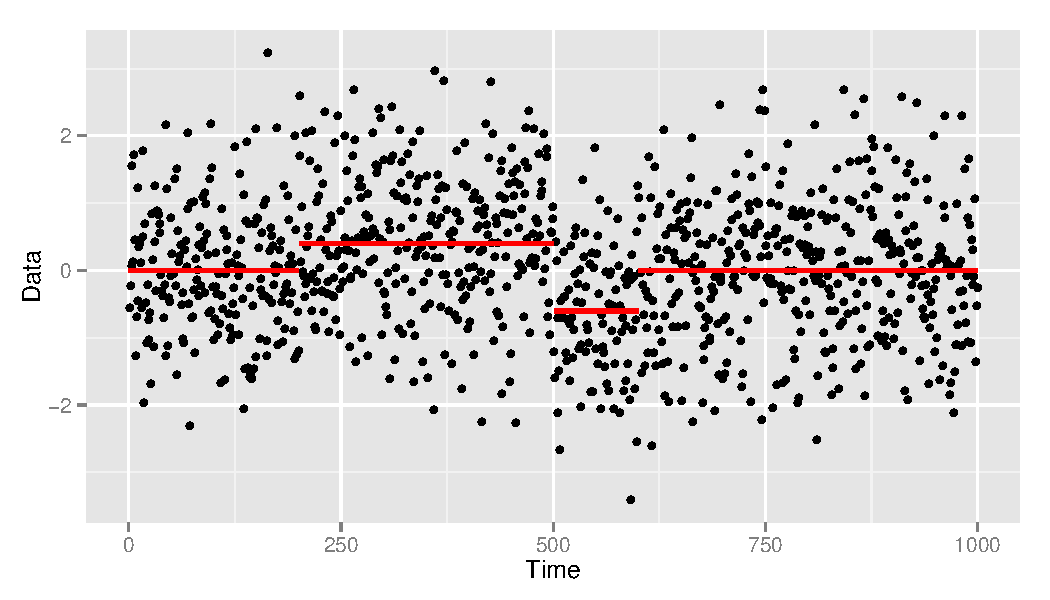
\includegraphics[width=\maxwidth]{figure/unnamed-chunk-2-1} 

}



\end{knitrout}

To generate the test statistics, we just use the snht function and pass in the time-series data.  Since this dataset is relatively simple, we don't need to worry much about the additional arguments.  We arbitrarily chose a period of 30; this specifies how many observations should be used to the left and right of a data point when computing the statistic.  A larger period, $P$, should give a better estimate of the statistic, but the statistic cannot be computed for the first and last $P$ observations.

\begin{knitrout}
\definecolor{shadecolor}{rgb}{0.969, 0.969, 0.969}\color{fgcolor}\begin{kframe}
\begin{alltt}
\hlkwd{library}\hlstd{(snht)}
\hlstd{snhtStatistic30} \hlkwb{=} \hlkwd{snht}\hlstd{(}\hlkwc{data} \hlstd{= baseData,} \hlkwc{period} \hlstd{=} \hlnum{30}\hlstd{)}
\hlkwd{summary}\hlstd{(snhtStatistic30)}
\end{alltt}
\begin{verbatim}
##      score            leftMean          rightMean       
##  Min.   : 0.0000   Min.   :-0.90009   Min.   :-0.90009  
##  1st Qu.: 0.1111   1st Qu.:-0.10870   1st Qu.:-0.14207  
##  Median : 0.5283   Median : 0.10943   Median : 0.10357  
##  Mean   : 1.6375   Mean   : 0.08714   Mean   : 0.07938  
##  3rd Qu.: 1.5264   3rd Qu.: 0.34558   3rd Qu.: 0.34558  
##  Max.   :40.4829   Max.   : 0.81457   Max.   : 0.81457  
##  NA's   :60        NA's   :60         NA's   :60
\end{verbatim}
\begin{alltt}
\hlstd{snhtStatistic60} \hlkwb{=} \hlkwd{snht}\hlstd{(}\hlkwc{data} \hlstd{= baseData,} \hlkwc{period} \hlstd{=} \hlnum{60}\hlstd{)}
\hlkwd{summary}\hlstd{(snhtStatistic60)}
\end{alltt}
\begin{verbatim}
##      score            leftMean          rightMean       
##  Min.   : 0.0000   Min.   :-0.72696   Min.   :-0.72696  
##  1st Qu.: 0.4049   1st Qu.:-0.08610   1st Qu.:-0.10620  
##  Median : 1.5558   Median : 0.11384   Median : 0.11249  
##  Mean   : 3.3498   Mean   : 0.09017   Mean   : 0.08557  
##  3rd Qu.: 3.2328   3rd Qu.: 0.32401   3rd Qu.: 0.32401  
##  Max.   :46.4891   Max.   : 0.62958   Max.   : 0.62958  
##  NA's   :120       NA's   :120        NA's   :120
\end{verbatim}
\end{kframe}
\end{knitrout}

And, here's a plot of the original data with the SNHT statistics computed above:

\begin{knitrout}
\definecolor{shadecolor}{rgb}{0.969, 0.969, 0.969}\color{fgcolor}\begin{kframe}
\begin{alltt}
\hlkwd{plotSNHT}\hlstd{(}\hlkwc{data} \hlstd{= baseData,} \hlkwc{stat} \hlstd{= snhtStatistic30,} \hlkwc{alpha} \hlstd{=} \hlnum{.05}\hlstd{)}
\end{alltt}
\end{kframe}

{\centering 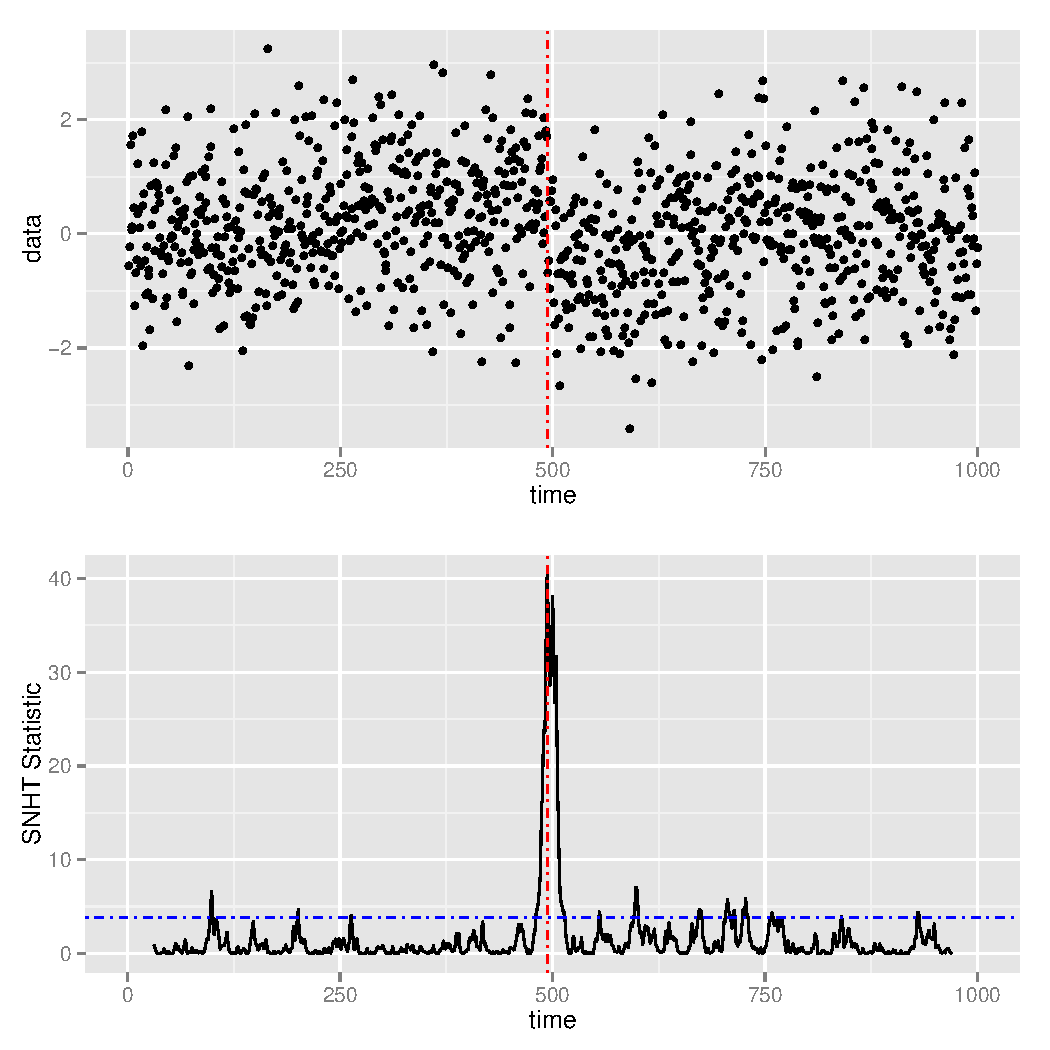
\includegraphics[width=\maxwidth]{figure/unnamed-chunk-4-1} 

}



\end{knitrout}

The red dashed vertical line represents the maximum SNHT statistic computed on the data.  If you are using the SNHT to homogenize data, you would shift the observations before this time by the difference in the two means at this point in time.  That difference is available from the test statistic object:

\begin{knitrout}
\definecolor{shadecolor}{rgb}{0.969, 0.969, 0.969}\color{fgcolor}\begin{kframe}
\begin{alltt}
\hlstd{largestStatTime} \hlkwb{=} \hlkwd{which.max}\hlstd{(snhtStatistic60}\hlopt{$}\hlstd{score)}
\hlstd{snhtStatistic60[largestStatTime, ]}
\end{alltt}
\begin{verbatim}
##        score  leftMean  rightMean
## 500 46.48912 0.5896035 -0.5740699
\end{verbatim}
\end{kframe}
\end{knitrout}

So, the observations to the left of 494 should be shifted by \ensuremath{-0.574} - 0.59 = \ensuremath{-1.164}.  Then, the SNHT statistic would be recomputed on this new dataset, and the process would repeat until no new statistic exceeds the threshold.  Note that we managed to find the largest break exactly, and our correction is close to the simulated error.

Under the null hypothesis of no changepoints and normal random errors, the test statistic follows a chi-squared distribution with one degree of freedom.  However, caution should be used if applying that threshold to all computed statistics simultaneously, as you then have the problem of multiple testing (and non-independent tests).  The blue dashed line in the plot above gives this threshold, but should be used with care.

We may also wish to compare the performance of the test with a longer period:

\begin{knitrout}
\definecolor{shadecolor}{rgb}{0.969, 0.969, 0.969}\color{fgcolor}\begin{kframe}
\begin{alltt}
\hlkwd{plotSNHT}\hlstd{(}\hlkwc{data} \hlstd{= baseData,} \hlkwc{stat} \hlstd{= snhtStatistic30,} \hlkwc{alpha} \hlstd{=} \hlnum{0.05}\hlstd{)}
\hlkwd{plotSNHT}\hlstd{(}\hlkwc{data} \hlstd{= baseData,} \hlkwc{stat} \hlstd{= snhtStatistic60,} \hlkwc{alpha} \hlstd{=} \hlnum{0.05}\hlstd{)}
\end{alltt}
\end{kframe}

{\centering 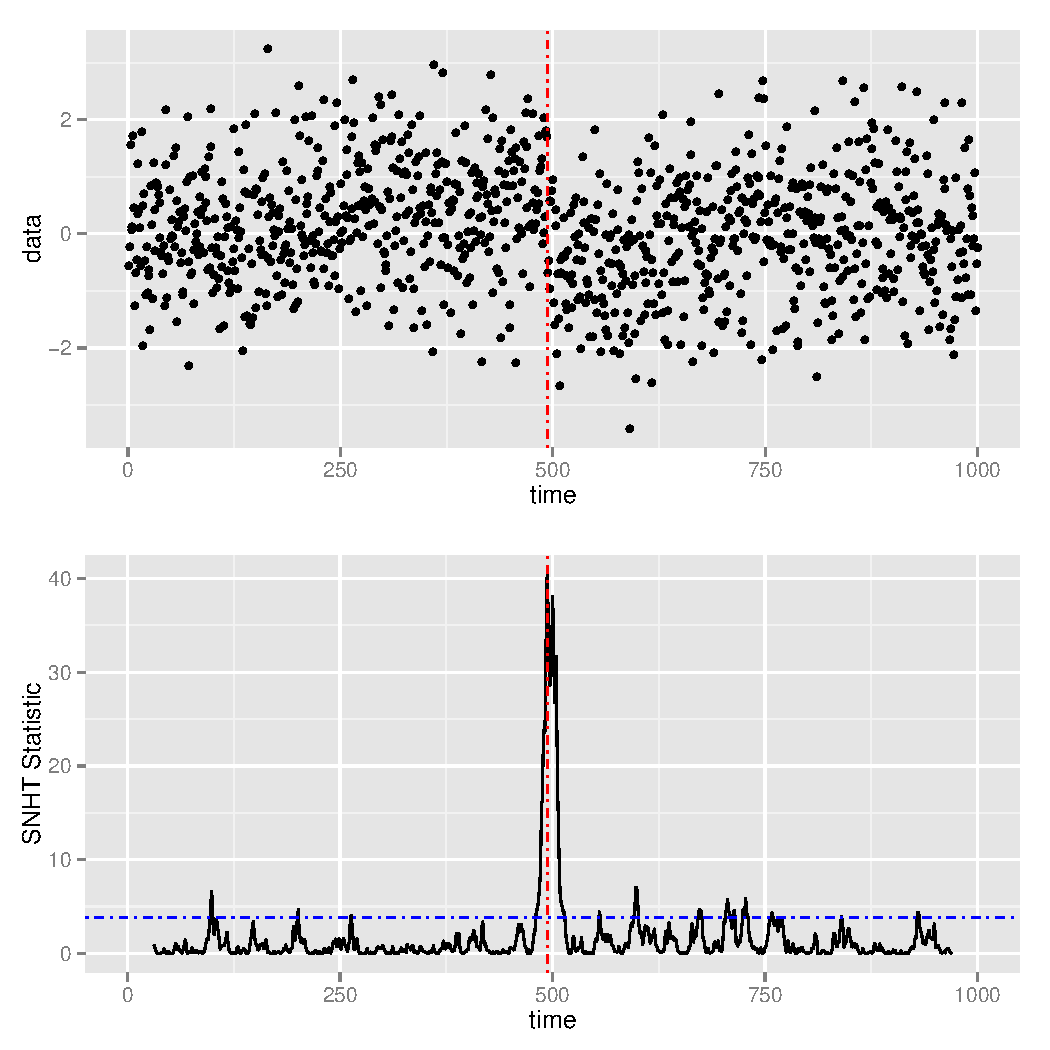
\includegraphics[width=\maxwidth]{figure/unnamed-chunk-6-1} 
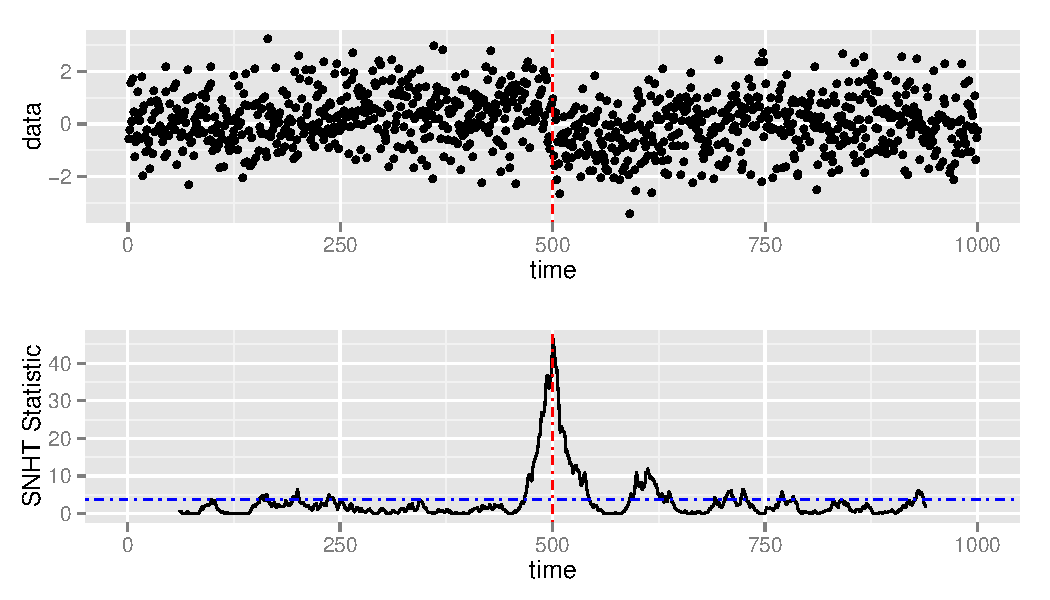
\includegraphics[width=\maxwidth]{figure/unnamed-chunk-6-2} 

}



\end{knitrout}

\subsection{Example 2: Seasonal trends, outliers, equal spacing in time}

Now, let's suppose that this data has a seasonal trend to it, as well as some outliers:

\begin{knitrout}
\definecolor{shadecolor}{rgb}{0.969, 0.969, 0.969}\color{fgcolor}\begin{kframe}
\begin{alltt}
\hlstd{seasonalData} \hlkwb{=} \hlstd{baseData} \hlopt{+} \hlkwd{cos}\hlstd{(}\hlnum{1}\hlopt{:}\hlnum{200} \hlopt{*} \hlnum{2} \hlopt{*} \hlstd{pi} \hlopt{/} \hlnum{200}\hlstd{)}
\hlstd{seasonalData} \hlkwb{=} \hlstd{seasonalData} \hlopt{+}
    \hlkwd{rbinom}\hlstd{(}\hlnum{1000}\hlstd{,} \hlkwc{p} \hlstd{=} \hlnum{.1}\hlstd{,} \hlkwc{size} \hlstd{=} \hlnum{1}\hlstd{)} \hlopt{*} \hlkwd{rnorm}\hlstd{(}\hlnum{1000}\hlstd{,} \hlkwc{sd} \hlstd{=} \hlnum{10}\hlstd{)}
\hlkwd{qplot}\hlstd{(}\hlnum{1}\hlopt{:}\hlnum{1000}\hlstd{, seasonalData)} \hlopt{+} \hlkwd{labs}\hlstd{(}\hlkwc{x} \hlstd{=} \hlstr{"Time"}\hlstd{,} \hlkwc{y} \hlstd{=} \hlstr{"Seasonal Data"}\hlstd{)}
\end{alltt}
\end{kframe}

{\centering 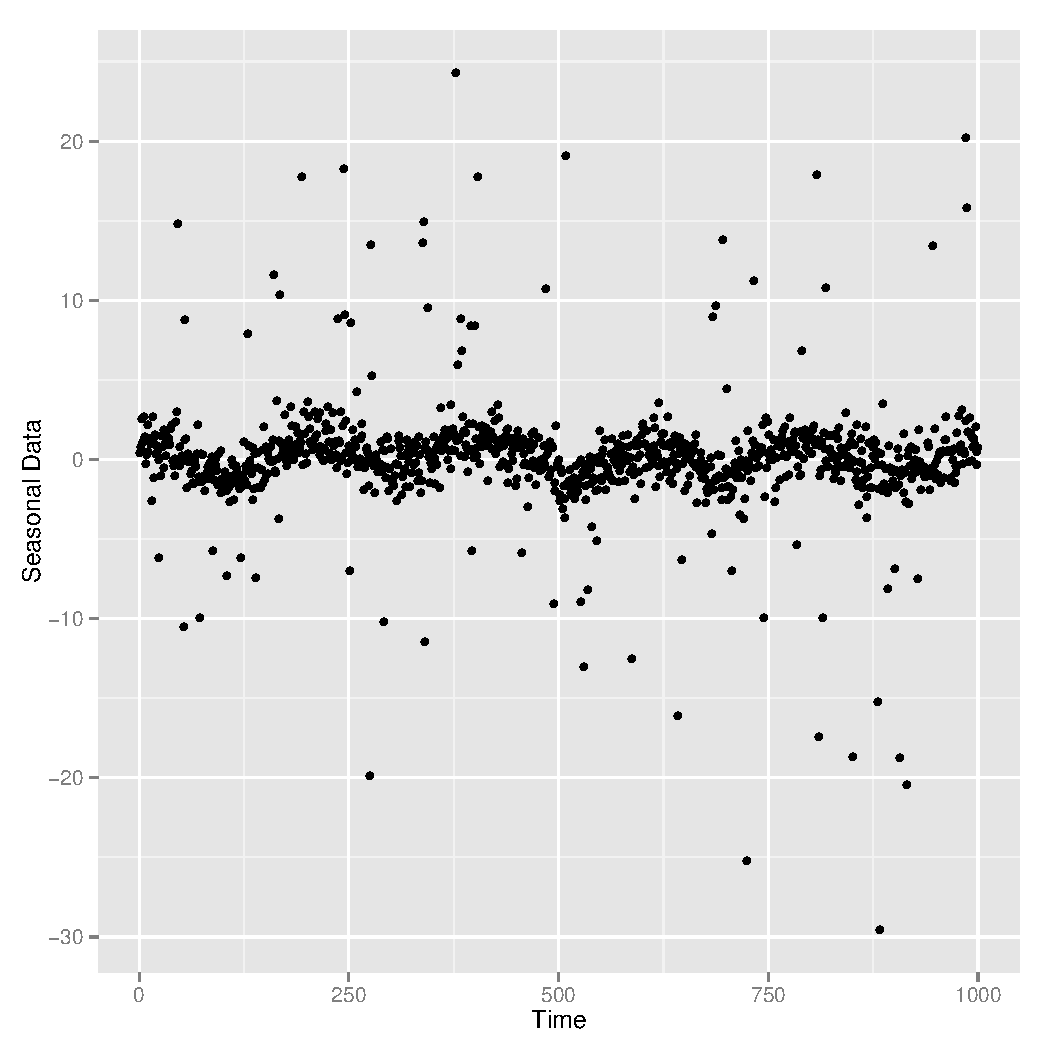
\includegraphics[width=\maxwidth]{figure/unnamed-chunk-7-1} 

}



\end{knitrout}

Now, the assumptions of the SNHT are invalid: we no longer have normal random errors about some mean.  We should use a period of 200 now, as we wish to average out the seasonal effects.

\begin{knitrout}
\definecolor{shadecolor}{rgb}{0.969, 0.969, 0.969}\color{fgcolor}\begin{kframe}
\begin{alltt}
\hlstd{snhtStatistic} \hlkwb{=} \hlkwd{snht}\hlstd{(}\hlkwc{data} \hlstd{= seasonalData,} \hlkwc{period} \hlstd{=} \hlnum{200}\hlstd{)}
\hlkwd{plotSNHT}\hlstd{(}\hlkwc{data} \hlstd{= seasonalData,} \hlkwc{stat} \hlstd{= snhtStatistic)}
\end{alltt}
\end{kframe}

{\centering 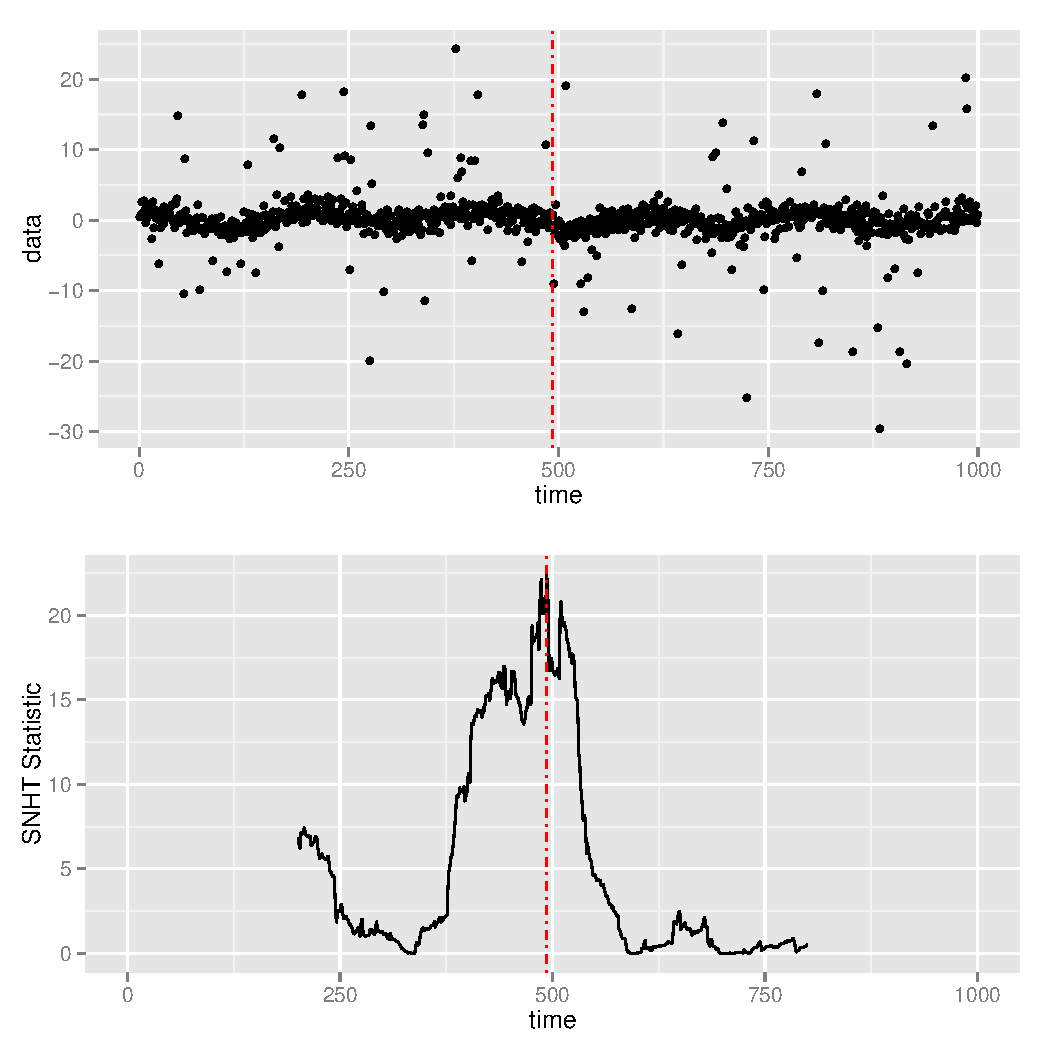
\includegraphics[width=\maxwidth]{figure/unnamed-chunk-8-1} 

}



\end{knitrout}

This statistic looks ok, but it completely fails to detect the third changepoint.  If we instead use the robust statistic, we see a smoother graph:

\begin{knitrout}
\definecolor{shadecolor}{rgb}{0.969, 0.969, 0.969}\color{fgcolor}\begin{kframe}
\begin{alltt}
\hlstd{snhtStatistic} \hlkwb{=} \hlkwd{snht}\hlstd{(}\hlkwc{data} \hlstd{= seasonalData,} \hlkwc{period} \hlstd{=} \hlnum{200}\hlstd{,} \hlkwc{robust} \hlstd{=} \hlnum{TRUE}\hlstd{,}
                     \hlkwc{rmSeasonalPeriod} \hlstd{=} \hlnum{200}\hlstd{)}
\hlkwd{plotSNHT}\hlstd{(}\hlkwc{data} \hlstd{= seasonalData,} \hlkwc{stat} \hlstd{= snhtStatistic)}
\end{alltt}
\end{kframe}

{\centering 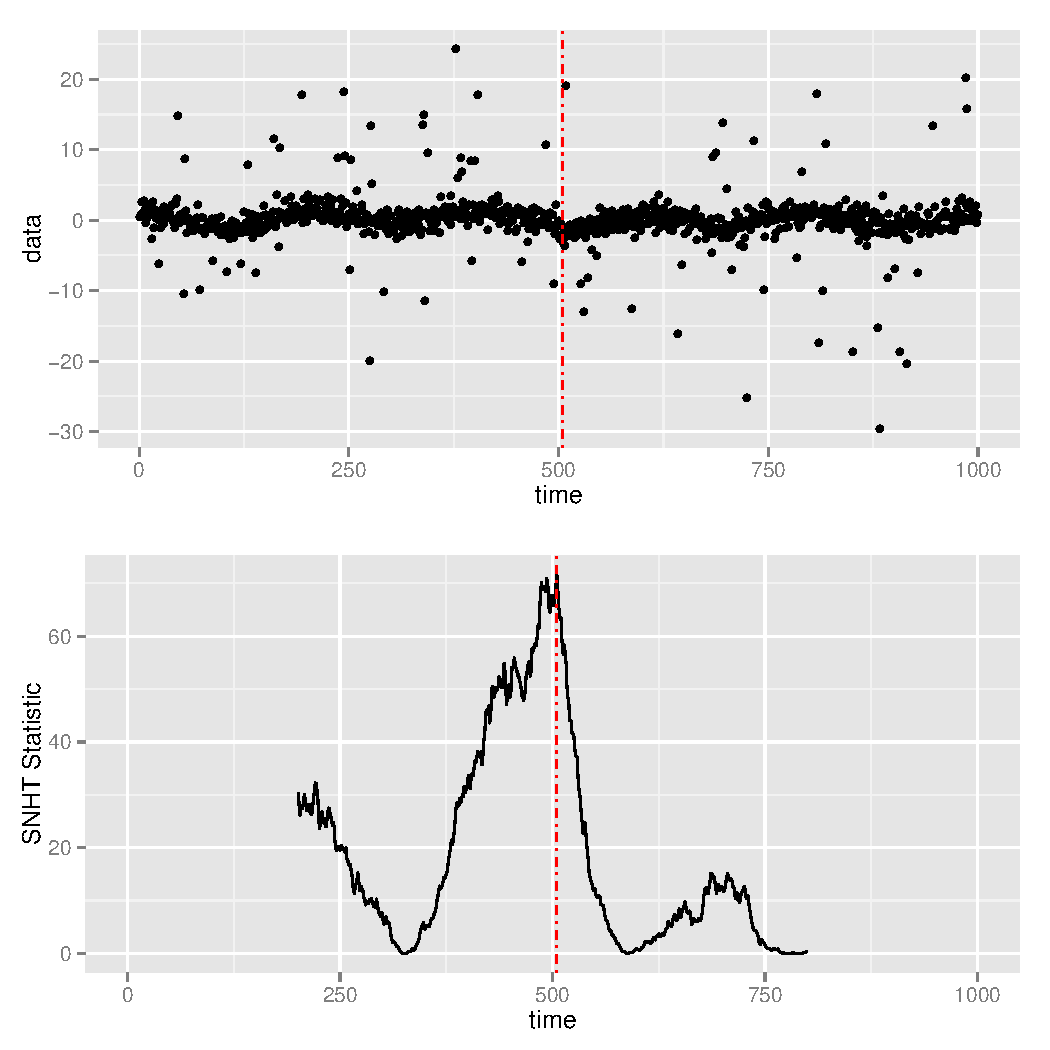
\includegraphics[width=\maxwidth]{figure/unnamed-chunk-9-1} 

}



\end{knitrout}

The statistic for the final break here is smaller than we'd hope for, but it's still present.

\subsection{Example 3: No seasonal trends, no outliers, unequal spacing in time}

Lastly, we may have observations that are unequally spaced in time.  The snht algorithm will handle these appropriately as long as we specify what times observations occurred at:

\begin{knitrout}
\definecolor{shadecolor}{rgb}{0.969, 0.969, 0.969}\color{fgcolor}\begin{kframe}
\begin{alltt}
\hlstd{times} \hlkwb{=} \hlnum{1}\hlopt{:}\hlnum{1000} \hlopt{+} \hlkwd{rnorm}\hlstd{(}\hlnum{1000}\hlstd{,} \hlkwc{sd} \hlstd{=} \hlnum{3}\hlstd{)}
\hlstd{times} \hlkwb{=} \hlkwd{sort}\hlstd{(times)}
\hlstd{snhtStatistic} \hlkwb{=} \hlkwd{snht}\hlstd{(}\hlkwc{data} \hlstd{= baseData,} \hlkwc{period} \hlstd{=} \hlnum{60}\hlstd{,} \hlkwc{time} \hlstd{= times)}
\hlkwd{summary}\hlstd{(snhtStatistic)}
\end{alltt}
\begin{verbatim}
##      score           leftMean          rightMean             time       
##  Min.   : 0.000   Min.   :-0.71899   Min.   :-0.71899   Min.   :  -2.0  
##  1st Qu.: 0.389   1st Qu.:-0.08560   1st Qu.:-0.10938   1st Qu.: 249.0  
##  Median : 1.626   Median : 0.11754   Median : 0.10382   Median : 500.5  
##  Mean   : 3.355   Mean   : 0.09156   Mean   : 0.08292   Mean   : 500.0  
##  3rd Qu.: 3.297   3rd Qu.: 0.31949   3rd Qu.: 0.32186   3rd Qu.: 751.2  
##  Max.   :46.242   Max.   : 0.61520   Max.   : 0.61625   Max.   :1005.0  
##  NA's   :112      NA's   :112        NA's   :112
\end{verbatim}
\end{kframe}
\end{knitrout}

Now, note that an additional column has been added to the snhtStatistic data.frame: time.  These times don't correspond exactly to the input times (as only one statistic is computed for each time step, for computational reasons).  We can again plot this new statistic:

\begin{knitrout}
\definecolor{shadecolor}{rgb}{0.969, 0.969, 0.969}\color{fgcolor}\begin{kframe}
\begin{alltt}
\hlkwd{plotSNHT}\hlstd{(}\hlkwc{data} \hlstd{= baseData,} \hlkwc{stat} \hlstd{= snhtStatistic,} \hlkwc{time} \hlstd{= times)}
\end{alltt}
\end{kframe}

{\centering 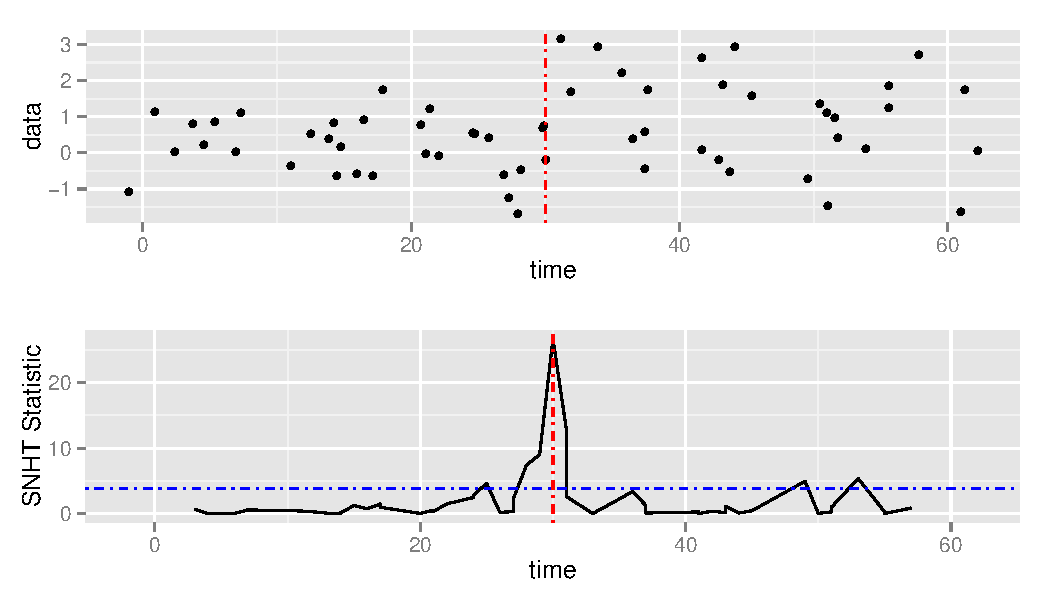
\includegraphics[width=\maxwidth]{figure/unnamed-chunk-11-1} 

}



\end{knitrout}

\bibliography{mybib}

\end{document}
